\documentclass[a4]{article}
\usepackage{geometry}
\geometry{a4paper,left=2cm,right=3cm, top=2cm, bottom=2cm} 
%\usepackage[austrian]{babel}
\renewcommand{\familydefault}{\sfdefault}
\usepackage{amsfonts,latexsym,amssymb,graphicx}
\usepackage{subfigure,epsfig,epstopdf}
%\usepackage{pdfsync}
\usepackage[utf8]{inputenc}
%\usepackage[T1]{fontenc}
\usepackage{booktabs} % For professional looking tables
\usepackage{multirow}
\usepackage{amsmath}

\usepackage[section]{placeins}

\title{\bf 183.605 \\ Machine Learning for Visual Computing \\ Assignment 1}
\author{Group 12: \\
	Hanna Huber (0925230) \\ Lena Trautmann (1526567) \\ Elisabeth Wetzer (0726681)}
\date{\today}


\begin{document}
\maketitle
\noindent

\begin{itemize}
\item Upload a zip-file with the required programs. You can choose the programming language.
\item Add a PDF document with answers to all of the questions of the assignment (particularly all required plots) and description and discussion of results. 
\end{itemize}

\section{Assignment 1}
\subsection{Part 1: Binary classification and the perceptron}

\subsubsection{Reading data}\label{sec:readdata}
%The file perceptrondata.csv contains 200 rows with 3 entries as ASCII-text. The left two columns represent the coordinates of two-dimensional observations. The right column holds the target-values  (1 oder -1) indicating the class assignments of the vectors.

\noindent {\bf Tasks:}
\begin{itemize}
\item Read the data using functions of your programming language resp. simulation software.
\end{itemize}
First, we wrote a new .csv-file with our .py-script to delete all extra blanks. Afterwards we could read in the data using \texttt{dlmread()}.

\begin{itemize}
\item Plot the input vectors in $\mathbb{R}^2$ and visualize corresponding target values (e.g. by using color). 
\end{itemize}
\begin{figure}[!h]
	\begin{center}
		\centering
		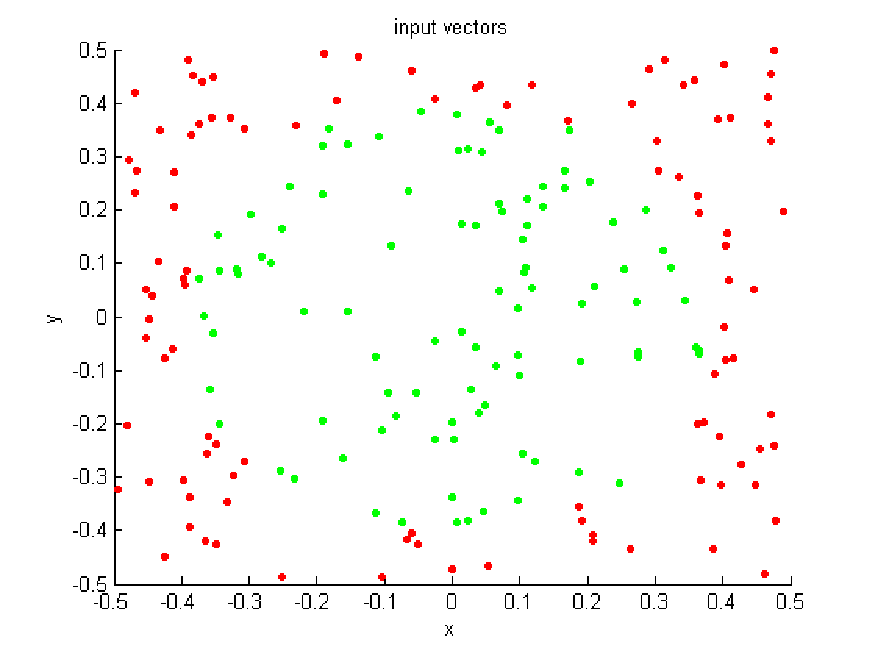
\includegraphics[width=6cm]{../figures/inputVectors.pdf}
	\end{center}	
	\caption{Plot of the input vectors with the target value visualized by colour.}
	\label{fig:inputVectors}
\end{figure}
Figure~\ref{fig:inputVectors} shows the input vectors.

\begin{itemize}
\item Use the feature transformation $(x_1,x_2) \rightarrow (x_1^2,x_2^2)$ and plot the data in the new feature space. The data should now be linearly separable.
\end{itemize}
\begin{figure}[!h]
	\begin{center}
		\centering
		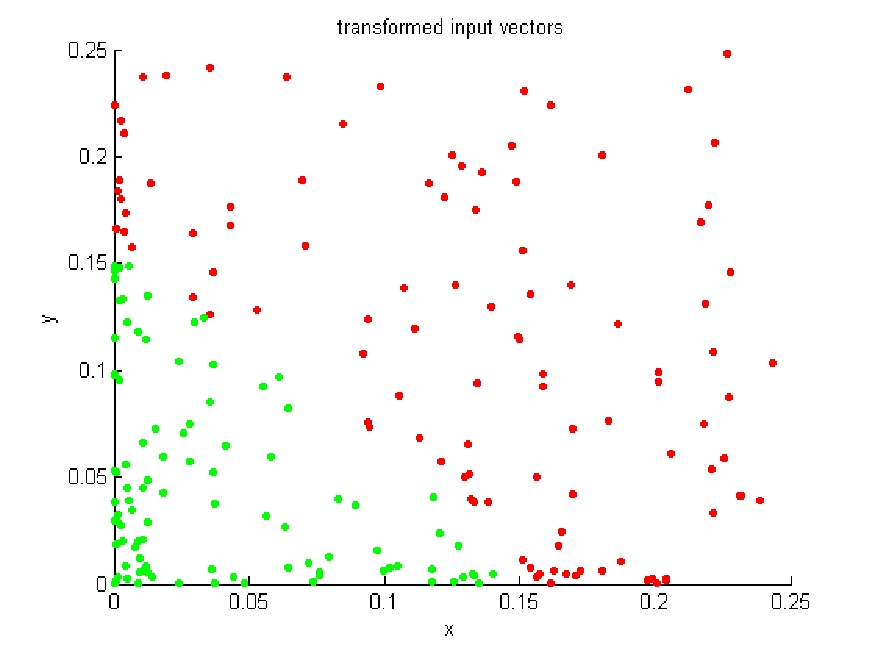
\includegraphics[width=6cm]{../figures/transformedInputVectors.pdf}
	\end{center}
	\caption{Plot of the transformed input vectors with the target value visualized by colour.}
	\label{fig:transformedInputVectors}
\end{figure}
Figure~\ref{fig:transformedInputVectors} shows the transformed input vectors.

\subsubsection{Perceptron training algorithm}
%The function
%\begin{center}
%\texttt{y = perc(w,X)}.
%\end{center}
%simulates a perceptron. The first argument is the weight vector ${\bf w}$ and the second argument is a matrix with input vectors in its columns ${\bf X}$. The output ${\bf y}$ is a binary vector with class labels 1 or -1.
%
%The function 
%\begin{center}
%\texttt{w = percTrain(X,t,maxIts,online)}.
%\end{center} 
%returns a weight vector ${\bf w}$ corresponding to the decision boundary separating the input vectors in ${\bf X}$ according to their target values ${\bf t}$.
%
%The argument $\texttt{maxIts}$ determines an upper limit for iterations of the gradient based optimization procedure. If this upper limit is reached before a solution vector is found, the function returns the current ${\bf w}$, otherwise it returns the solution weight vector. \texttt{online} is \emph{true} if the \emph{online}-version of the optimization procedure is to be used or \emph{false} for the \emph{batch}-version. 
%\vspace{2mm}
%

\noindent {\bf Tasks:}
\begin{itemize}
\item Implement both functions. Use homogeneous coordinates and the corresponding augmented weight vector ${\mathbf w}\in\mathbb{R}^3$.
\end{itemize}
The functions \texttt{percTrain} and \texttt{perc} are implemented in the files \texttt{percTrain.m} and \texttt{perc.m}, respectively.
\begin{itemize}
	\item Plot the data and decision boundary in $\mathbb{R}^2$, both in the original data space (see e.g. Figure~\ref{fig:perceptron}) and in the feature space of basis functions, each at three different stages of the training: after the first iteration, after approximately half of the required iterations, and after convergence.
\end{itemize}
\begin{figure}[!h]
	\begin{center}
		\centering
		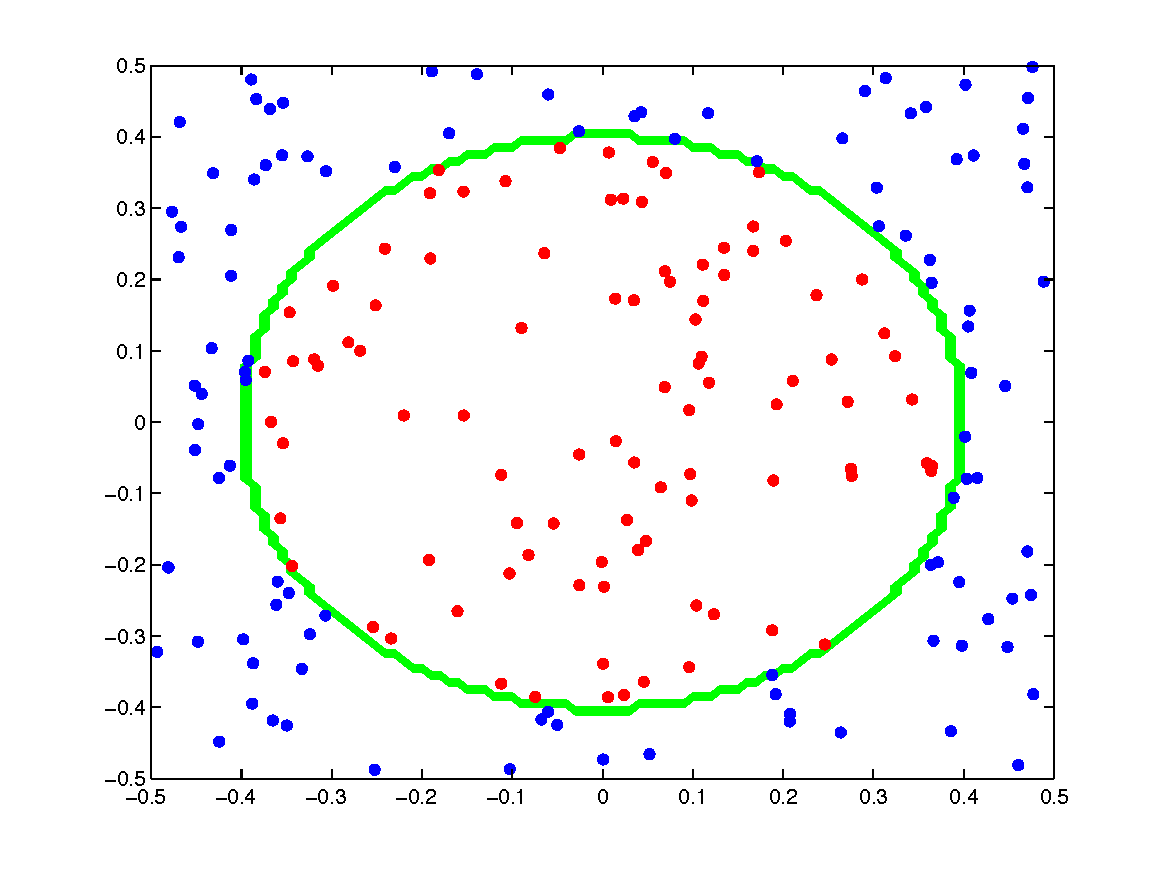
\includegraphics[width=6cm]{../figures/perceptron.pdf}
	\end{center}
	\caption{\label{fig:perceptron}Plot of the decision boundary in the original data space found by the perceptron (green curve) together with labelled data points.}
\end{figure}
Figures~\ref{fig:origOL},~\ref{fig:transOL},~\ref{fig:origBA},~\ref{fig:transBA} show perceptron learning after the first iteration, half of the iterations needed and after the final iteration. They show that the algorithm converges much faster using online learning (see Figures~\ref{fig:origOL} and~\ref{fig:transOL}). Figures~\ref{fig:transOL} and~\ref{fig:transBA} illustrate how the transformation into the feature space of basis functions makes the data linearly separable. The non-linear decision boundary in the original data space is obtained by applying the inverse transformation to the linear decision boundary in feature space.
\begin{figure}[h!]
\centering
	\subfigure[]{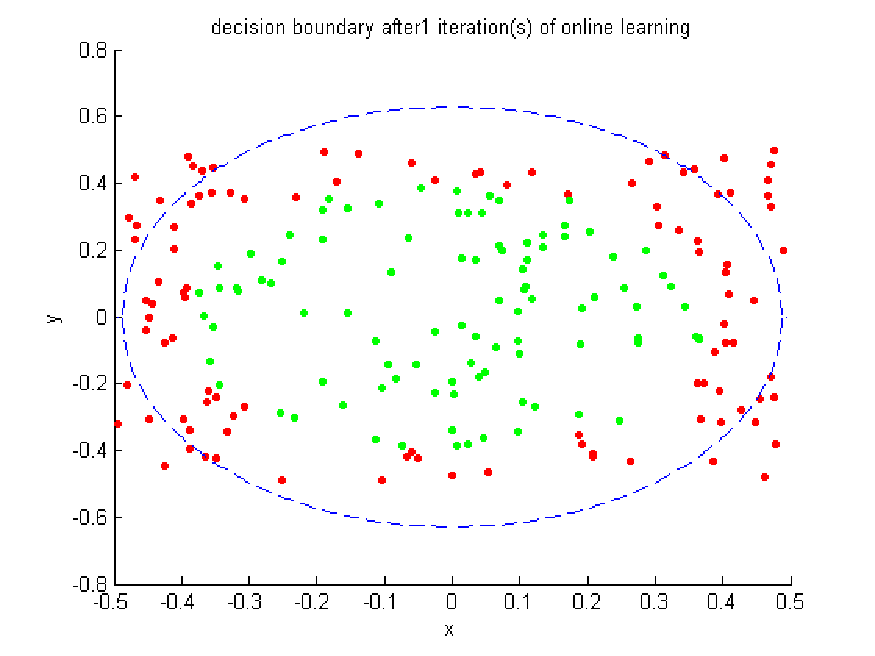
\includegraphics[width=5cm]{../figures/originalOnlineIt1.pdf}}
	\subfigure[]{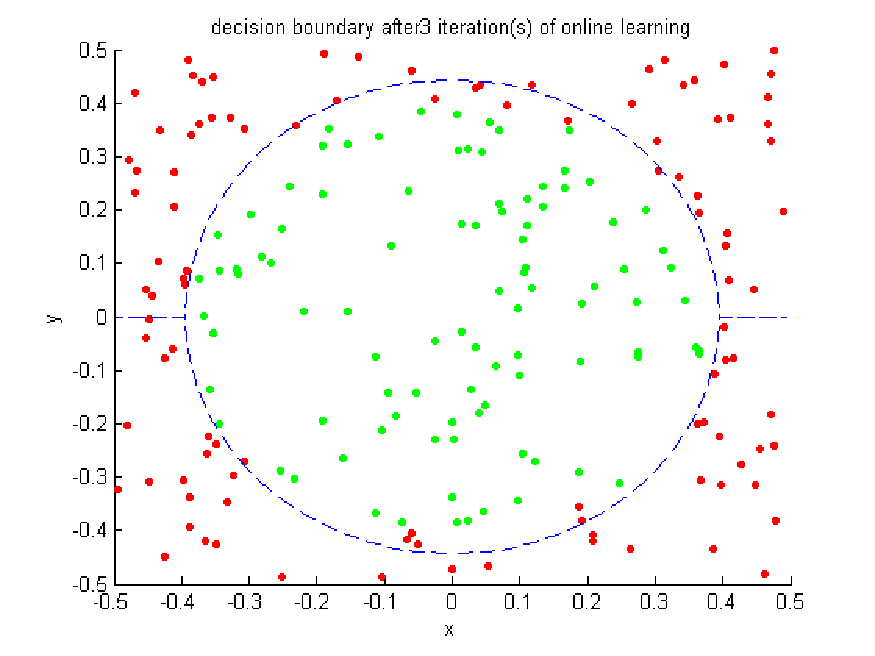
\includegraphics[width=5cm]{../figures/originalOnlineIt3.pdf}}
	\subfigure[]{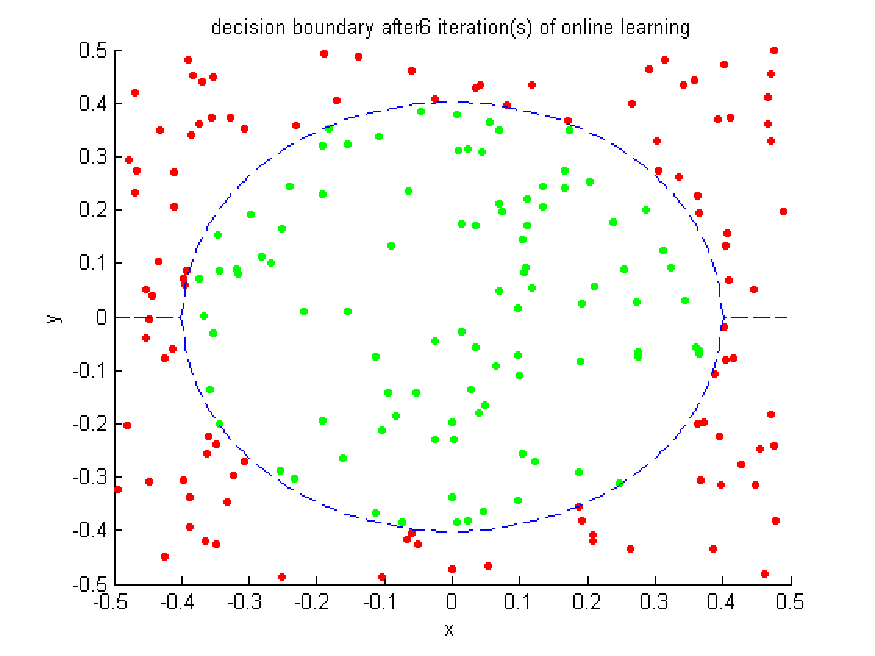
\includegraphics[width=5cm]{../figures/originalOnlineIt6.pdf}}
\caption{Perceptron decision boundary in the original data space at iterations \#1, \#3 and \#6 of online learning.}
\label{fig:origOL}
\end{figure}
\begin{figure}[h!]
\centering
	\subfigure[]{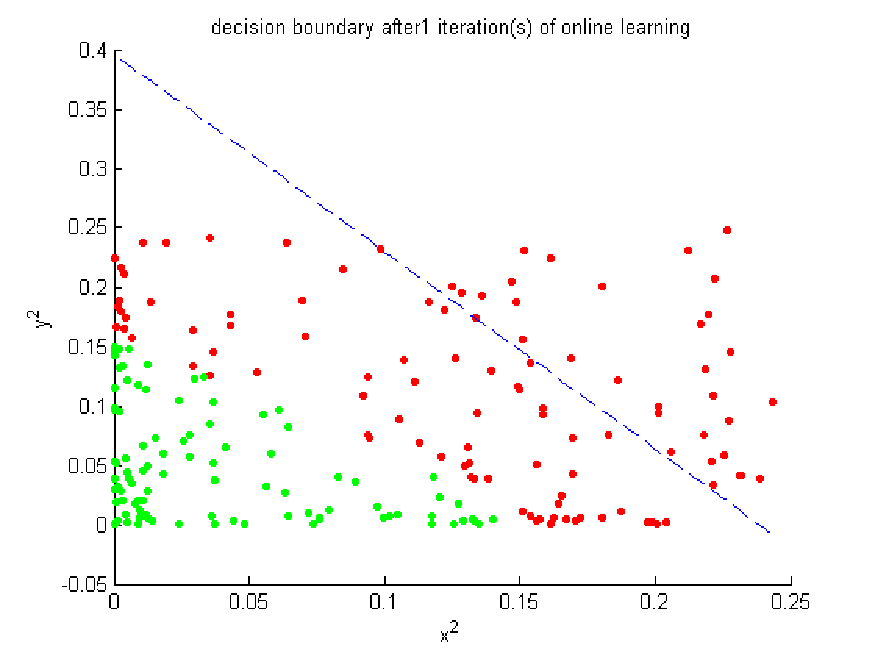
\includegraphics[width=5cm]{../figures/transformedOnlineIt1.pdf}}
	\subfigure[]{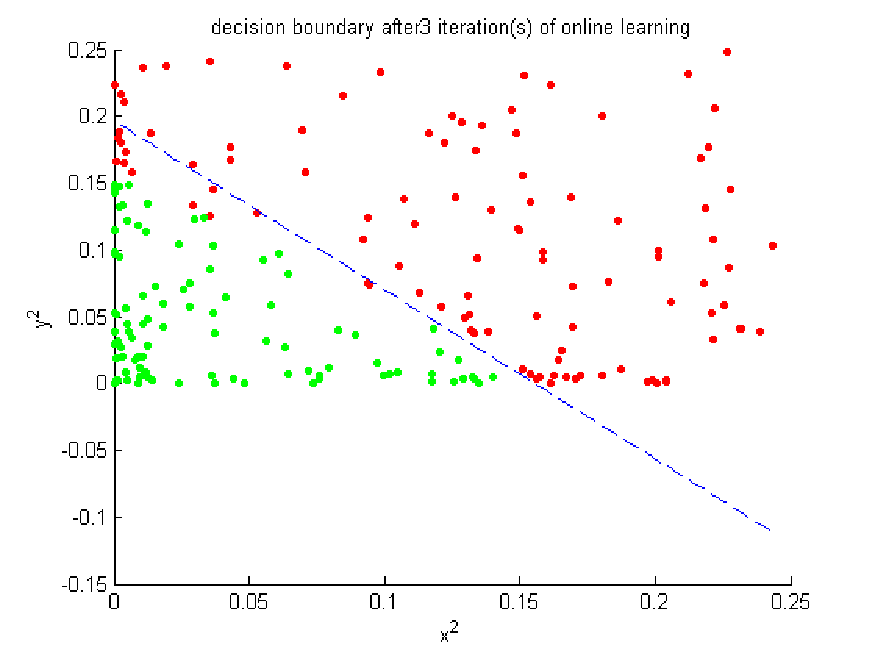
\includegraphics[width=5cm]{../figures/transformedOnlineIt3.pdf}}
	\subfigure[]{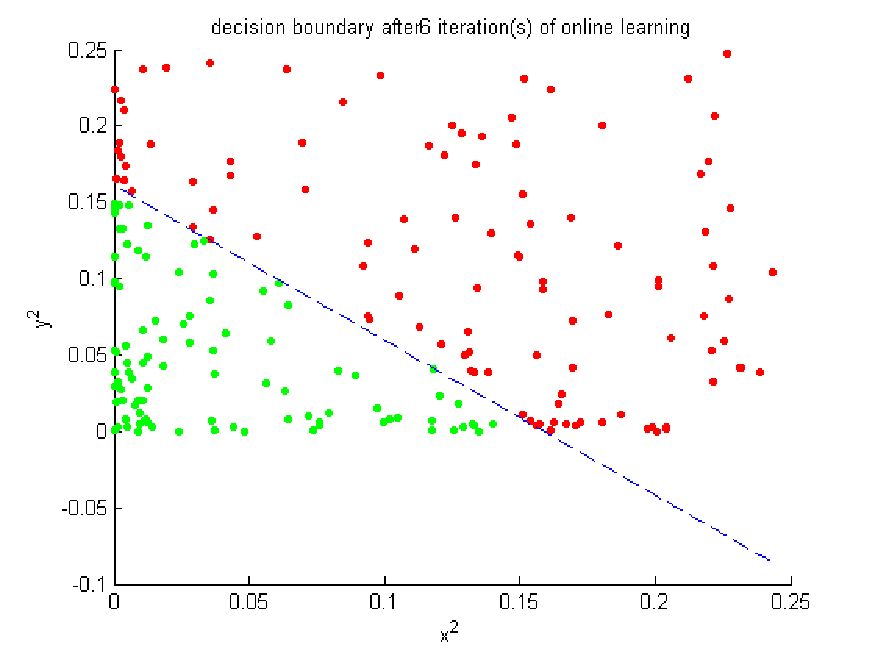
\includegraphics[width=5cm]{../figures/transformedOnlineIt6.pdf}}
\caption{Perceptron decision boundary in the feature space of basis functions at iterations \#1, \#3 and \#6 of online learning.}
\label{fig:transOL}
\end{figure}
\begin{figure}[h!]
\centering
	\subfigure[]{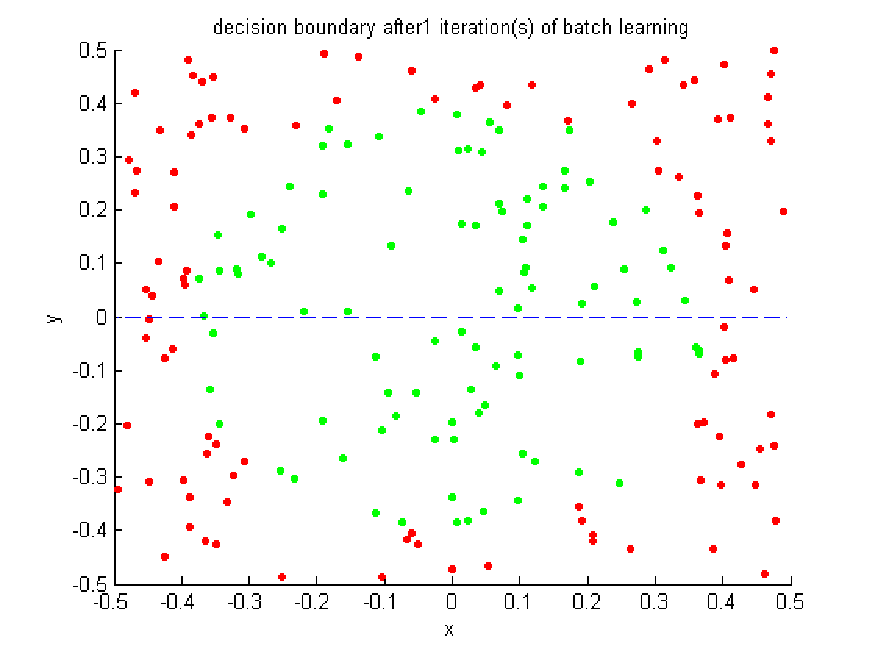
\includegraphics[width=5cm]{../figures/originalBatchIt1.pdf}}
	\subfigure[]{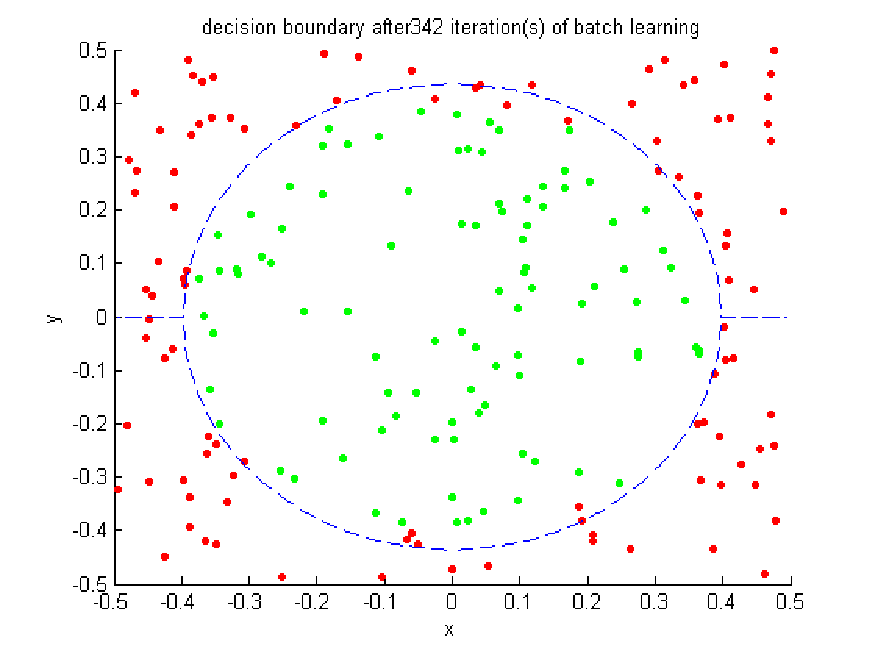
\includegraphics[width=5cm]{../figures/originalBatchIt342.pdf}}
	\subfigure[]{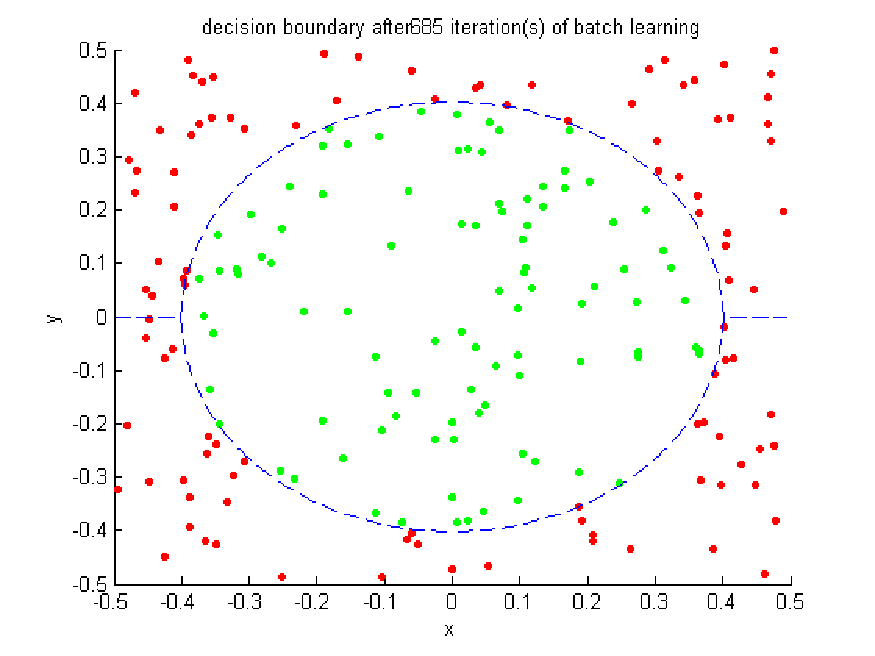
\includegraphics[width=5cm]{../figures/originalBatchIt685.pdf}}
\caption{Perceptron decision boundary in the original data space at iterations \#1, \#342 and \#685 of batch learning.}
\label{fig:origBA}
\end{figure}
\begin{figure}[h!]
\centering
	\subfigure[]{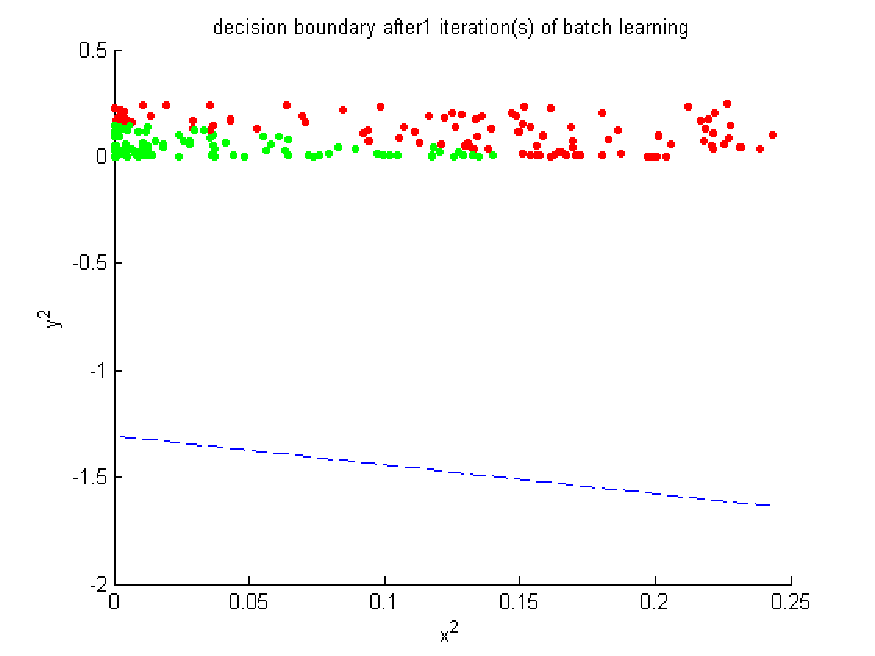
\includegraphics[width=5cm]{../figures/transformedBatchIt1.pdf}}
	\subfigure[]{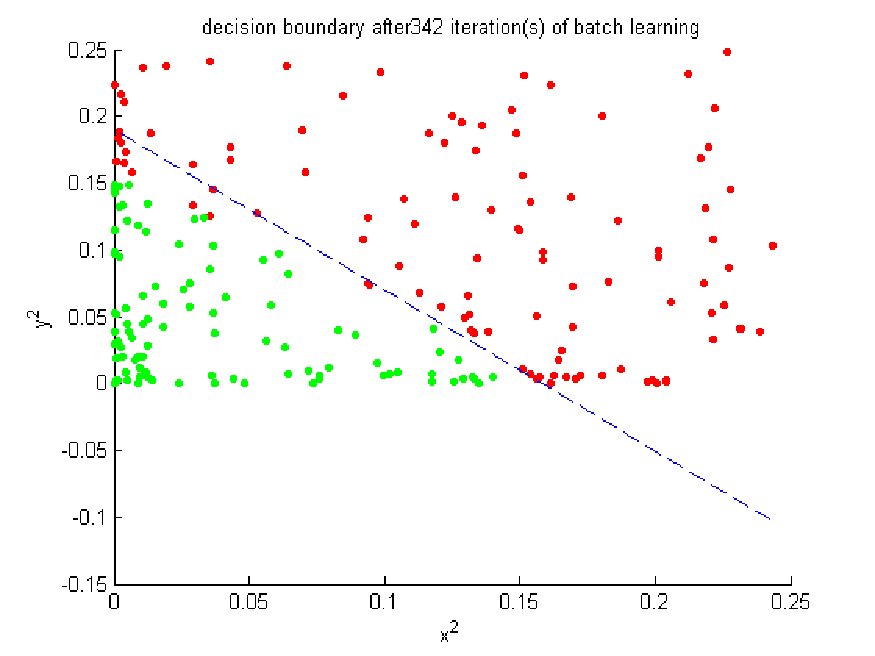
\includegraphics[width=5cm]{../figures/transformedBatchIt342.pdf}}
	\subfigure[]{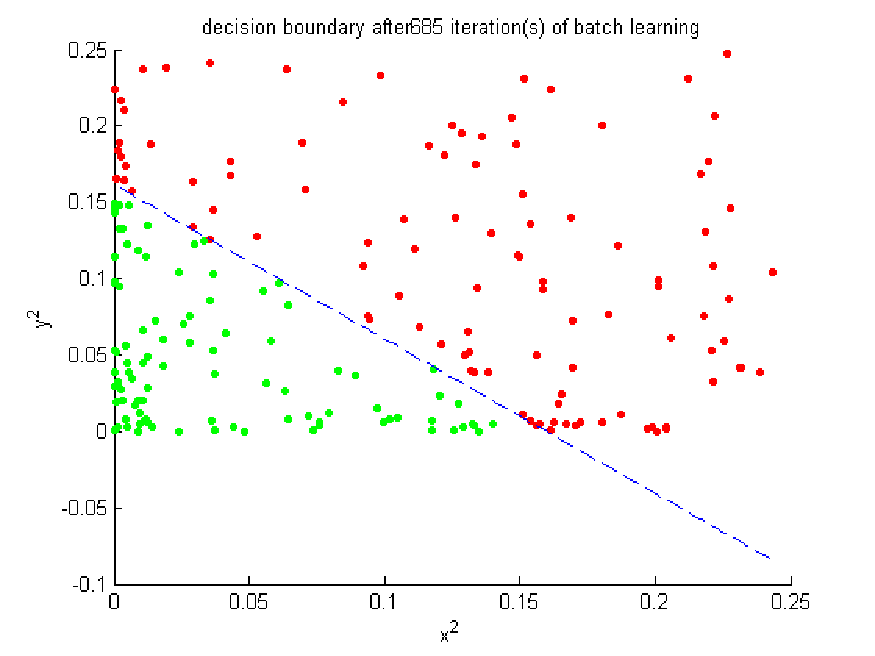
\includegraphics[width=5cm]{../figures/transformedBatchIt685.pdf}}
\caption{Perceptron decision boundary in the feature space of basis functions at iterations \#1, \#342 and \#685 of batch learning.}
\label{fig:transBA}
\end{figure}
\begin{itemize}
\item Initialize ${\bf w} = {\bf 0}$. What is the influence of the learning rate?
\end{itemize}
The weight vector is initialized as ${\bf w} = {\bf 0}$. This way, the learning rate $\gamma$ merely scales the weight vector ${\bf w^{(j)}} = \gamma \sum_{i\in M}x_it_i$, where $j$ denotes the current iteration and $M$ the set of data points that have been misclassified and used to update {\bf w} up to this point. As $(\gamma_1 \sum_{i\in M}x_it_i)^T (x_kt_k) \leq 0 \Leftrightarrow  (\gamma_2 \sum_{i\in M}x_it_i)^T (x_kt_k) \leq 0$ for any $\gamma_1, \gamma_2 > 0$, the classification of the $k$th data point and thus the learning behaviour of the perceptron are not influenced by the learning rate.

\FloatBarrier
\subsection{Part 2: Linear basis function models for regression}

%Aim of this exercise to deepen understanding of parameter optimization of error function while taking into account the relation of model complexity (in this case it corresponds to the number of basis functions used) and the expected error. Since this expected value (the mean squared error) is a theoretical quantity, it has to be estimated by the average of the error of predictions resulting from many training runs with different randomly generated target values.

\subsubsection{Experimental setup}
%A row vector of scalar inputs $x \in [0,5]$ sampling the interval in steps of $0.1$ (resulting in 51 values) and a corresponding output vector $\mathbf{y}$ with values $y = f(x) = 2x^2-Gx+1$ is the basis of this experiment. The coefficient $G$ is your group number. These 51 points are to be used for the visualization of the target function and the predictions of the fitted model.
%A training set is generated by subsampling the 51 values as follows: Every eighth value ($x_0 = 0$, $x_1 = 0.8$, $x_2 = 0.16$, ...) is assigned to the training set and the target values $t_i$ are obtained by adding to the corresponding $y_i$ a random value from the normal distribution $\mathcal{N}(\mu = 0,\sigma = 16)$. Thus, the training set contains $N = 9$ pairs of observations $x_i, t_i$. 
%
%We will employ a linear basis function model of the form $f_{\mathbf w}(x) = {\mathbf w}^T{\mathbf \Phi}(x)$, where\begin{equation} \nonumber
%{\mathbf \Phi}(x) \rightarrow \left(
%\begin{array}{c} 1\\ x \\ x^2 \\ \vdots \\ x^d \\ \end{array}\right),
%\end{equation} 
%and ${\mathbf w} \in \mathbb{R}^{d+1}$. The model will be fitted to the training set by minimization of the training error 
%\begin{equation}
%E({\mathbf w}) = \sum_{i = 1}^N(t_i - {\mathbf w}^T{\mathbf \Phi}(x_i))^2
%\end{equation} 
%also known as the \emph{residual sum of squares} (RSS). The optimal weight vector is given by ${\mathbf w}^* = \arg\min_{\mathbf w} E({\mathbf w})$.
%
%
%\begin{figure}[!h]
%\begin{center}
%\centering
%	\subfigure[]{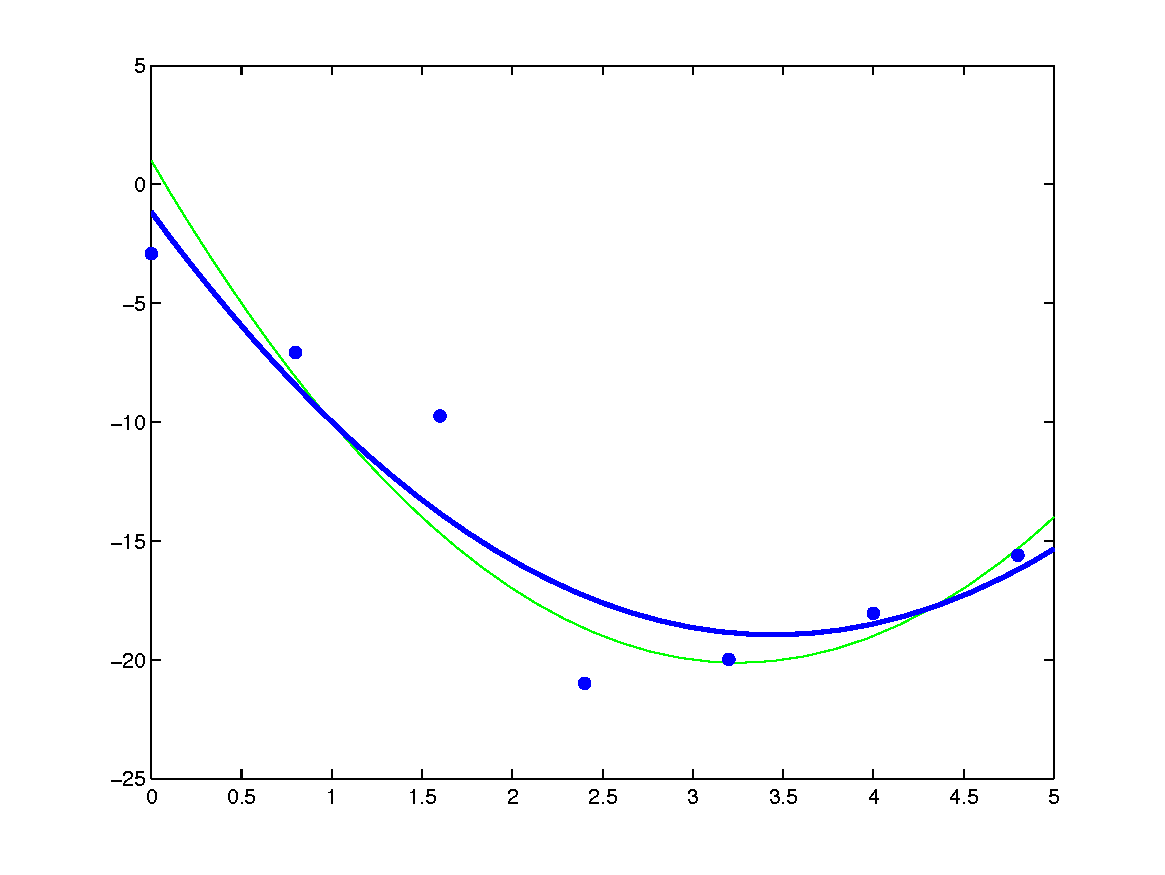
\includegraphics[width=5.5cm]{../figures/regressiond2.pdf}}
%	\subfigure[]{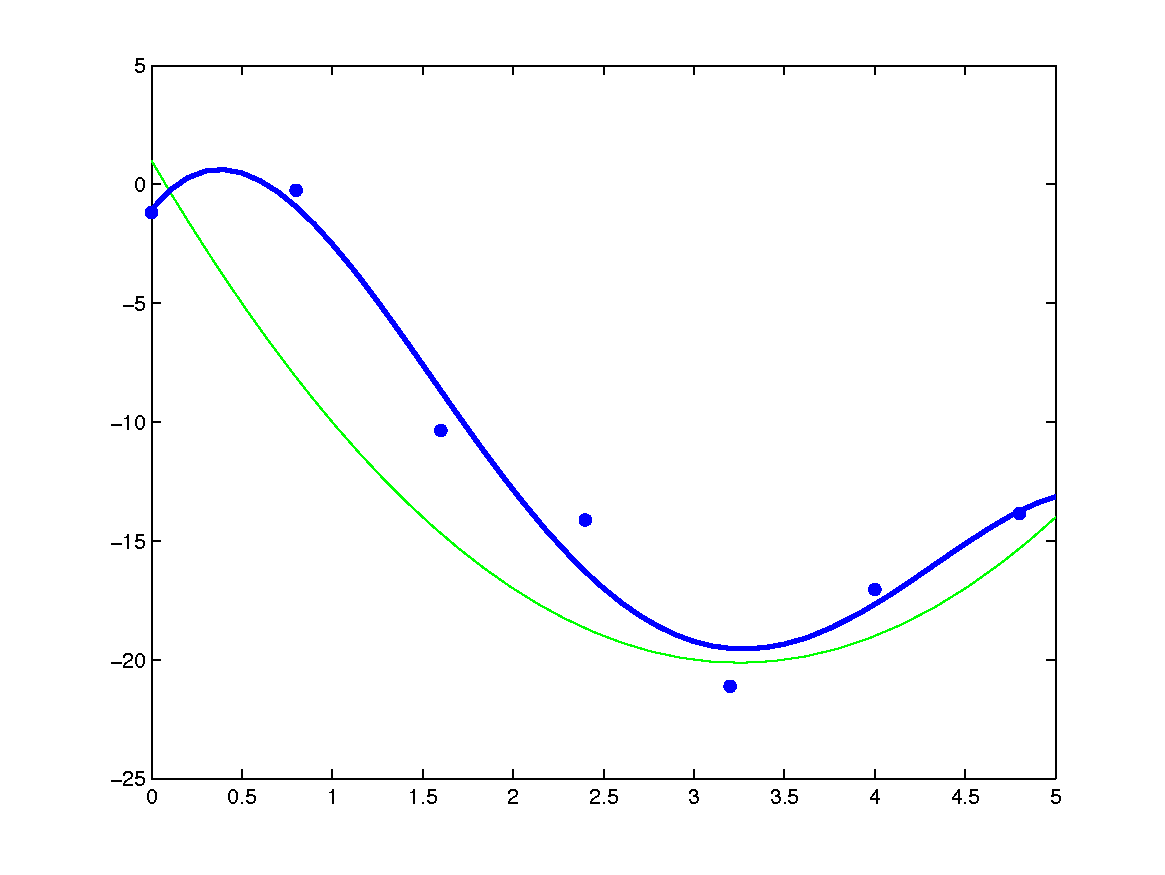
\includegraphics[width=5.5cm]{../figures/regressiond4.pdf}}
%\end{center}
%\caption{An example of a true target function (thin green curve) from which the training data was generated, training set (without feature transformation) with $N=9$ (blue dots) and prediction of the fitted model ${\mathbf w}^T{\mathbf \Phi}(x)$ (blue curve). The basis functions are ${\mathbf \Phi}(x) \rightarrow (1,x,x^2,x^3,...,x^d)^T$. (a) $d=2$ (b) $d=4$.}
%\end{figure}
At the end of the setup we have:
\begin{itemize}
	\item xtrain and ttrain: the training data
	\item phi: the transformation function
	\item xtrain\_phi: the transformation of xtrain
\end{itemize} 

\subsubsection{Optimization: \emph{LMS}-learning rule vs. closed form}
%
%Use a linear unit (\emph{online} LMS-learning rule) for regression on transformed input data. In a first step use a linear basis function model with $d=2$ (in Matlab you can calculate the power elementwise: e.g. \texttt{[x x x].$\wedge$ [0 1 2]}). Hint: Visualize $y$ and its prediction during the training or observe the chance of the weight vector to determine useful values for $\gamma$.
%\vspace{2mm}
%
\noindent {\bf Tasks:}
\begin{itemize}
	\item What is the resulting weight vector when using the LMS-rule?
\end{itemize}
\begin{table} [tbp!]
	\caption{Weight vector derived for the LMS-rule (online and closed form)}
	\centering
	\label{table:wLMS}
	\begin{tabular}{l c c c}
		\toprule
		& $\phi_0$ & $\phi_1$ & $\phi_2$ \\ 
		\midrule
		wOnline & -2.4164  & -6.7862  &  0.7742 \\
		wClosed &  -2.4193  & -6.7593  &  0.7645  \\
		\bottomrule
	\end{tabular}
\end{table}
\begin{figure}[!h]
	\centering
	\subfigure[\label{fig:122_LMS_online}]{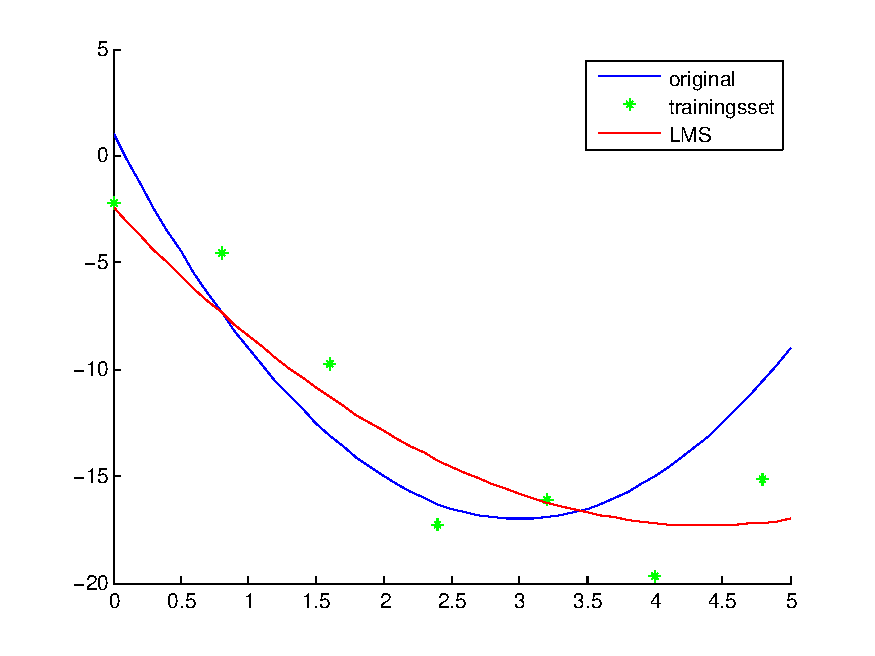
\includegraphics[width=6cm]{../figures/LMS.pdf}}
	\subfigure[\label{fig:122_LMS_closed}]{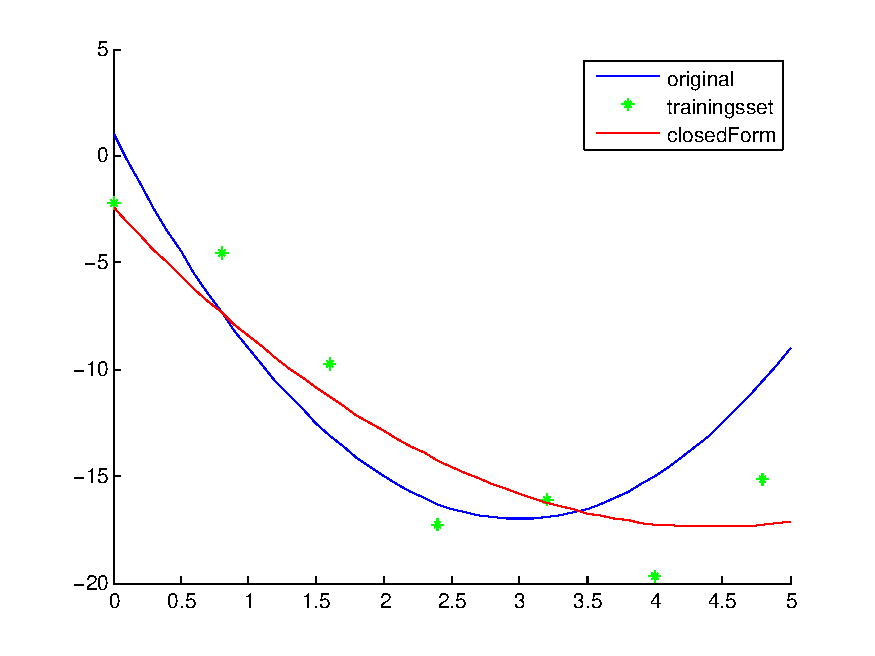
\includegraphics[width=6cm]{../figures/closed.pdf}}
	\caption{Optimization using the LMS-rule with online learning (a) and in closed form (b)}
	\label{fig:122_LMS}
\end{figure}
The values of the resulting weight vector is summarized in Table~\ref{table:wLMS} and the corresponding curve plotted in Figure~\ref{fig:122_LMS_online}.

\begin{itemize}
	\item How can you determine the optimal ${\mathbf w}^*$ in closed form? Compare ${\mathbf w}^*$ with the outcome of the LMS-rule training.
\end{itemize}
The closed form is calculated by updating the weight vector, determined by all N points, in one step. The resulting values are also summarized in Table~\ref{table:wLMS} and the corresponding curve plotted in Figure~\ref{fig:122_LMS_closed}.
\begin{itemize}	
	\item What is the influence of $\gamma$? Which value for $\gamma$ represents a good tradeoff between number of iterations and convergence? 
\end{itemize}
The learning rate $\gamma$ controls the influence of the single data points. Using high learning rates during online learning,  the regression reacts quickly and moves towards the current data point. This is disadvantageous if the current data point is an outlier. Consequently, if the learning rate is too high, the number of iterations until convergence increases as well. The same problem occurs, if the rate is too low and the regression reacts too slowly. For this assignment, we observed that a learning rate of $\gamma=0.0001$ is a suitable choice. \\
Also, the difference between online and batch learning decreases with decreasing values of $\gamma$. This is due to the fact that the weight vector $\bf{w}$ only changes very little with each data point during online learning. As a result, the update factor for subsequent datapoints is also only slightly changed. This way, the difference between adding the update factors subseuqently or at the same time is less remarkable. \\

\subsubsection{Model-complexity and model-selection}
Determine ${\mathbf w}^*$ in closed form for 2000 different training sets, in which only the $t_i$ are varyied according to $\mathcal{N}(\mu = y_i,\sigma = 4)$, while the $x_i$ remain unchanged. \\
Assuming that a deterministic function $y(\mathbf{x}, \mathbf{w})$ specifies the target variable $t$. Varying the only the $t_i$ according to $\mathcal{N}(\mu = y_i,\sigma = 4)$, we get $t=y(\mathbf{x}, \mathbf{w}) + \epsilon$, where $\epsilon$ is a random variable $\sim \mathcal{N}(\mu = 0,\sigma = 16)$.\\
We get
$$p(t| \mathbf{x}, \mathbf{w}, \frac{1}{16}) = \mathcal{N}(t|y(\mathbf{x}, \mathbf{w}), 4)$$
The sum of squares error function is definied as in \cite{Bishop}:
$$E(\mathbf{w})=\frac{1}{2} \sum_{n=1} ^N (t_n- \mathbf{w}^T \mathbf{\phi}(\mathbf{x_n}))^2$$
To minimize the error function, the gradient is set to zero:
$$\sum_{n=1}^N t_n \mathbf{\phi}(\mathbf{x}_n)^T- \mathbf{w}^T \left( \sum_{n=1} ^N \mathbf{\phi} ( \mathbf{x}_n) \mathbf{\phi} ( \mathbf{x}_n)^T \right)=0$$
Hence the solution for $\mathbf{w}$ is obtained by:
$$ \mathbf{w}=(\mathbf{X}^T\mathbf{X})^{-1}\mathbf{X}^T\mathbf{t}$$
where the entries of $\mathbf{X} \in \mathbb{R}^{N \times M}$ are given by $\phi_j(\mathbf{x}_n)$. \\
$(\mathbf{X}^T\mathbf{X})^{-1}\mathbf{X}^T$ is known to be the Moore-Penrose-inverse of $\mathbf{X}$ and can be calculated in Matlab by \verb+pinv(X)+. \\

\vspace{2mm}
\noindent {\bf Tasks}\footnote{In all tasks $\mathcal{E}$ refers to the expected value with respect to the random variable ${\mathbf w^*}$, i.e. $\mathcal{E} \equiv \mathcal{E}_{\mathbf w^*}$}:
\begin{itemize}
\item Select a fixed $x'$, which is not an observation of the training set, but lies between two observations. In the following trials $x' = 2$ was chosen.
\item Estimate the \emph{mean squared error} 
\begin{equation} \nonumber
\mbox{\emph{mse}} = \mathcal{E} (f(x')-f_{\mathbf w^*}(x'))^2,
\end{equation}i.e., the mean of the squared residuals of the models prediction $f_{\mathbf w^*}(x')$ from the true function value $f(x')$ for all $0 \leq d \leq 8$ ($d = 0$ corresponds to a constant function) using at least 2000 trials.  
\item Estimate by the same way the quantities \emph{bias}$^2 = (f(x')-\mathcal{E} f_{\mathbf w^*}(x'))^2$ and \emph{var}$ =\mathcal{E} (f_{\mathbf w^*}(x') - \mathcal{E} f_{\mathbf w^*}(x'))^2$.
\item Plot \emph{mse}, \emph{bias}$^2$ and \emph{var} against $d$ together in one plot. What is the relation of the quantities?
\item (optional) Generate the above plots only for $d=8$, but minimize instead of $E({\mathbf w})$ the regularized error function 
\begin{equation}
E_{\lambda}({\mathbf w}) = \sum_{i = 1}^N(t_i - {\mathbf w}^T{\mathbf \Phi}(x_i))^2 + \lambda \|{\mathbf w}\|^2,
\end{equation} 
i.e. ${\mathbf w}^* = \arg\min_{\mathbf w}^* E_{\lambda}({\mathbf w})$. Plot the quantities against $\lambda$ instead of $d$. Hint: The minimum can be obtained in closed form (see lecture slides). 
\end{itemize}


The expected value of the mean squared error $\mathcal{E} (f(x')-f_{\mathbf w^*}(x'))^2$ for two thousand trials evaluated at $x'=2$ is plotted against $d$, the number of dimensions of the linear basis function space in blue in figure \ref{fig:NonReg}. The same plot shows the bias $ (f(x')-\mathcal{E} f_{\mathbf w^*}(x'))^2$ and the variance $\mathcal{E} (f_{\mathbf w^*}(x') - \mathcal{E} f_{\mathbf w^*}(x'))^2$ in red and yellow respectively.
As described in \cite{hastie} the expected squared error on a sample x can be decomposed by the bias and variance as follows:
$$\mathcal{E} (f(x')-f_{\mathbf w^*}(x'))^2=(f(x')-\mathcal{E} f_{\mathbf w^*}(x'))^2+\mathcal{E} (f_{\mathbf w^*}(x') - \mathcal{E} f_{\mathbf w^*}(x'))^2 +\epsilon$$
where $\epsilon$ is an irreducible error.\\

\begin{figure}[!h]
	\begin{center}
		\centering
		\includegraphics[width=6cm]{../figures/NonReg}
		%\includegraphics[width=0.5\textwidth]{NonReg}
	\end{center}
	\caption{\label{fig:NonReg} The expected value of the mean squared error, the bias and the variance against $d$ for a fixed $x'=2$ evaluated for 2000 trials, where $d$ denotes the dimension of the basis functions model}
\end{figure}

This relationship is seen in figure \ref{fig:NonReg}. In higher dimensions than $d=2$ the bias becomes zero and the expected mean squared error is equal to the variance estimate. Furthermore table \ref{table:EvalD} lists the model qualities in dependence of $d$. The last column shows that the mean squared error can be decomposed into the given bias and variance up to an accuracy of $10^{-13}$, which relates to the irreducible error $\epsilon$.
The plots in figure \ref{fig:NonReg} are conclusive with the literature: dimensionality reduction can decrease variance, but simplicity of the model introduces more bias, while adding features to the model decreases the bias, but in return increases the variance. 
The mean squared error shows a minimum at $d=2$. The spike in the plot can be explained by the fact that the quantities were calculated for one explicit $x$ and would average out by taking the average of multiple evaluation points of the trials.

\begin{table} [h]
	\caption{Estimated MSE, Variance and Bias of non-regularized Model}
	\centering
	\label{table:EvalD}
	\begin{tabular}{c c c c c}
		\toprule
		d &MSE &  Bias &  Variance  & MSE-(Bias+Variance)\\ 
		\midrule
		0& 17.51&  15.09 &  2.42   & 1.0e-13 *-0.96\\
		1& 26.07&  23.49  &  2.57 & 1.0e-13 * 0.60 \\
		2& 5.34&  1.10 & 5.34  &1.0e-13 * 0.07 \\
		3& 6.02&  6.63  & 6.02  & 1.0e-13 * 0.10 \\
		 4& 8.26&  0.00 &  8.26  & 1.0e-13 * 0.23 \\
		 5&11.18&  0.00  &  11.17  & 1.0e-13 *-0.05  \\
		 6& 12.60& 0.00  &  12.60  & 1.0e-13 * 0.16 \\
		7&12.14&  0.00  &  12.14 & 1.0e-13 *-0.28\\
		8& 12.99 &  0.00 &   12.98  & 1.0e-13 *-0.21 \\
		\bottomrule
	\end{tabular}
\end{table}

In order to control overfitting a regularization term is often added to the error function which shall be minimized to find an optimal solution. Instead of minimizing $E(\mathbf{w})=\frac{1}{2} \sum_{n=1} ^N (t_n- \mathbf{w}^T \mathbf{\phi}(\mathbf{x_n}))^2$, the modified error function $\tilde{E}(\mathbf{w})=\frac{1}{2} \sum_{n=1} ^N (t_n- \mathbf{w}^T \mathbf{\phi}(\mathbf{x_n}))^2 + \frac{1}{2} \lambda \mathbf{w}^T \mathbf{w}$ is to be minimized. There are other options to choose a regularizer than $\lambda || \mathbf{w} ||$ but it is a simple choice to demonstrate the trade off between bias and variance. This specific regularizer is called weight decay and does not effect the circumstance of the error function being quadratic and hence convex. Setting the gradient of the error function in respect to $\mathbf{w}$ to zero gives:
$$\mathbf{w}=(\lambda \mathbf{I} + \mathbf{X}^T \mathbf{X})^{-1}\mathbf{X}^Tt$$
where $\mathbf{I}$ denotes the identity matrix.
As before the expected mean squared error, the bias and the variance are plotted, but only for dimension $d=8$, which introduced a large variance in the non-regularized model. Figure \ref{fig:Reg} shows the quantities against $\lambda$, where $\lambda$ is chosen to be $\exp (i-4)$, where $i$ is the index on the x-axis in the figure. For small $\lambda$ the variance dominates the mean squared error, because the model complexity is high. For greater $\lambda$, hence greater regularization, the variance is restrained, but in exchange to an increase in bias. The results of the tests are shown in table \ref{table:EvalD}. The decomposition of the mean squared error into the bias and variance terms leaves an error as small as $10^{-12}$.


\begin{figure}[!h]
	\begin{center}
		\centering
		\includegraphics[width=6cm]{../figures/Reg}
		%\includegraphics[width=0.5\textwidth]{Reg}
	\end{center}
	\caption{\label{fig:Reg}The expected value of the mean squared error, the bias and the variance against the index of $\lambda$ for a fixed $x'=2$ evaluated for 2000 trials, where $\lambda$ denotes the weight decay parameter and is considered $\exp ( \text{index} - 4)$}
\end{figure}




\begin{table} [h]
	\caption{Estimated MSE, Variance and Bias of regularized Model}
	\centering
	\label{table:EvalD}
	\begin{tabular}{c c c c c}
		\toprule
		$\lambda$ & MSE &  Bias &  Variance  & MSE-(Bias+Variance)\\ 
		\midrule
		 $\exp(-3)$ & 10.70&  0.04 &  10.66   & 1.0e-12 *-0.01\\
		 $\exp(-2)$ & 10.44&  0.08  &  10.36 & 1.0e-12 *-0.04 \\
		 $\exp(-1)$ & 10.25&  0.07 & 10.17  &1.0e-12 *  0.02 \\
		 1 & 9.90&  0.03  & 9.87  & 1.0e-12 * 0.01 \\
		 $\exp(1)$ &  9.23&  0.02 & 9.21  & 1.0e-12 * 0.01 \\
		 $\exp(2)$ & 8.64&  0.83  &  7.81 & 1.0e-12 * 0.01  \\
		 $\exp(3)$ &  12.08& 6.62  &  5.46  & 1.0e-12 *-0.15 \\
		$\exp(4)$ & 28.04&  25.03  &  3.01 & 1.0e-12 *-0.16\\
		\bottomrule
	\end{tabular}
\end{table}






 \bibliography{lit}
 \bibliographystyle{unsrt}





\end{document}
